\hyperdef{sums}{asymptotics}{\chapter{Sums \& Asymptotics}}\label{asymptotics_chap}

\iffalse

\begin{staffnotes}

\section*{Closed Forms and Approximations}

Sums and products arise regularly in the analysis of algorithms and in
other technical areas such as finance and probabilistic systems.  We've
already seen that
\[
\sum_{i=1}^n i = \frac{n(n+1)}{2}.
\]
Having a simple \emph{closed form} expression such as $n(n+1)/2$ makes the
sum a lot easier to understand and evaluate.  We proved by induction that
this formula is correct, but not where it came from.  In
Section~\ref{findsum_sec}, we'll discuss ways to find such closed forms.  Even
when there are no closed forms exactly equal to a sum, we may still be
able to find a closed form that \emph{approximates} a sum with useful
accuracy.

The product we focus on in this chapter is the familiar factorial:
\[
n!\  \eqdef\ \ 1 \cdot 2 \cdots  (n-1) \cdot n  = \prod_{i=1}^n i.
\]
We'll describe a closed form approximation for it called \emph{Stirling's
Formula}.

Finally, when there isn't a good closed form approximation for some
expression, there may still be a closed form that characterizes its growth
rate.  We'll introduce \emph{asymptotic notation}, such as ``big Oh'', to
describe growth rates.

\end{staffnotes}
\fi

\hyperdef{value}{annuity}{\section{The Value of an
    Annuity}}\label{annuity_sec}

Would you prefer a million dollars today or \$50,000 a year for the
rest of your life?  On the one hand, instant gratification is nice.
On the other hand, the total dollars received at \$50K per year is
much larger if you live long enough.

Formally, this is a question about the value of an annuity.  An
\term{annuity} is a financial instrument that pays out a fixed amount of
money at the beginning of every year for some specified number of years.
In particular, an $n$-year, $m$-payment annuity pays $m$ dollars at the
start of each year for $n$ years.  In some cases, $n$ is finite, but not
always.  Examples include lottery payouts, student loans, and home
mortgages.  There are even Wall Street people who specialize in trading
annuities.

A key question is what an annuity is worth.  For example, lotteries often
pay out jackpots over many years.  Intuitively, $\$50,000$ a year for 20
years ought to be worth less than a million dollars right now.  If you had
all the cash right away, you could invest it and begin collecting
interest.  But what if the choice were between $\$50,000$ a year for 20
years and a \emph{half} million dollars today?  Now it is not clear which
option is better.

In order to answer such questions, we need to know what a dollar paid out
in the future is worth today.  To model this, let's assume that money can
be invested at a fixed annual interest rate $p$.  We'll assume an 8\%
rate\footnote{U.S. interest rates have dropped steadily for several years,
  and ordinary bank deposits now earn around 1.5\%.  But just a few years
  ago the rate was 8\%; this rate makes some of our examples a little more
  dramatic.  The rate has been as high as 17\% in the past thirty
  years.

  In Japan, the standard interest rate is near zero\%, and on a few
  occasions in the past few years has even been slightly negative.  It's a
  mystery why the Japanese populace keeps any money in their banks.}  for
the rest of the discussion.

Here is why the interest rate $p$ matters.  Ten dollars invested today
at interest rate $p$ will become $(1+p)\cdot 10 = 10.80$ dollars in a
year, $(1+p)^2\cdot 10 \approx 11.66$ dollars in two years, and so
forth.  Looked at another way, ten dollars paid out a year from now
are only really worth $1/(1+p) \cdot 10 \approx 9.26$ dollars today.
The reason is that if we had the $\$9.26$ today, we could invest it
and would have $\$10.00$ in a year anyway.  Therefore, $p$ determines
the value of money paid out in the future. 

\subsection{The Future Value of Money}

So for an $n$-year, $m$-payment annuity, the first payment of $m$ dollars
is truly worth $m$ dollars.  But the second payment a year later is worth
only $m/(1+p)$ dollars.  Similarly, the third payment is worth
$m/(1+p)^2$, and the $n$-th payment is worth only $m/(1+p)^{n-1}$.  The
total value, $V$, of the annuity is equal to the sum of the payment
values.  This gives:
\begin{align}
  V & = \sum_{i=1}^n \frac{m}{(1+p)^{i-1}}\notag\\
  & = m \cdot \sum_{j=0}^{n-1} \paren{\frac{1}{1+p}}^j & \text{(substitute $j \eqdef i-1$)}\notag\\
  & = m \cdot \sum_{j=0}^{n-1} x^j \quad (\mbox{substitute} \ x =
  \frac{1}{1+p}).\label{jn-1xsum}
\end{align}
The summation in~\eqref{jn-1xsum} is a \idx{geometric sum} that has a
\term{closed form}, making the evaluation a lot easier, namely\footnote{To
  make this equality hold for $x=0$, we adopt the convention that $0^0
  \eqdef 1$.},
\begin{equation}\label{geometric-sum-n-1}
\sum_{i=0}^{n-1} x^i = \frac{1- x^n}{1 - x}.
\end{equation}
(The phrase ``closed form'' refers to a mathematical expression without
any summation or product notation.)

Equation~\eqref{geometric-sum-n-1} was proved by induction in
problem~\ref{CP_geometric_series_induction}, but, as is often the case,
the proof by induction gave no hint about how the formula was found in the
first place.  So we'll take this opportunity to explain where it comes
from.  The trick is to let $S$ be the value of the sum and then observe
what $-xS$ is:
\[\begin{array}{rclllllcl}
  S & = & 1 & +  x & + x^2 & + x^3 & + &\cdots & + x^{n-1} \\
-xS & = &   & -  x & - x^2 & - x^3 & - &\cdots & - x^{n-1} - x^{n}.
\end{array}\]
Adding these two equations gives:
\begin{align*}
S-xS  & =  1 - x^n, \\
\intertext{  so}
S     & = \frac{1 - x^n}{1 - x}.
\end{align*}
We'll look further into this method of proof in a few weeks when we
introduce \emph{generating functions} in 
Chapter 16.%~\ref{generating_function_chap}.


\subsection{Closed Form for the Annuity Value}
So now we have a simple formula for $V$, the \idx{value of an
  annuity} that pays $m$ dollars at the start of each year for $n$ years.
\begin{align}
  V & = m \frac{1 - x^n}{1-x}
      & \text{(by~\eqref{jn-1xsum} and~\eqref{geometric-sum-n-1})}\label{Vmfrac1x}\\
  & = m \frac{1 + p - \paren{1/(1+p)}^{n-1}}{p}
      & (x = 1/(1+p)).\label{annval1p}
\end{align}
The formula~\eqref{annval1p} is much easier to use than a summation with
dozens of terms.  For example, what is the real value of a winning lottery
ticket that pays $\$50,000$ per year for 20 years?  Plugging in $m =
\$50,000$, $n = 20$, and $p = 0.08$ gives $V \approx \$530,180$.  So
because payments are deferred, the million dollar lottery is really only
worth about a half million dollars!  This is a good trick for the lottery
advertisers!

\subsection{Infinite Geometric Series}

The question we began with was whether you would prefer a million dollars
today or $\$50,000$ a year for the rest of your life.  Of course, this
depends on how long you live, so optimistically assume that the second
option is to receive $\$50,000$ a year \emph{forever}.  This sounds like
infinite money!  But we can compute the value of an annuity with an
infinite number of payments by taking the limit of our geometric sum
in~\eqref{geometric-sum-n-1} as $n$ tends to infinity.
\begin{theorem}\label{th:series}
If $\abs{x} < 1$, then
\[
\sum_{i=0}^\infty x^i = \frac{1}{1-x}.
\]
\end{theorem}

\begin{proof}
\begin{align*}
\sum_{i=0}^\infty x^i
   & \eqdef  \lim_{n \rightarrow \infty} \sum_{i=0}^{n-1} x^i \\
   & = \lim_{n \rightarrow \infty} \frac{1 - x^n}{1-x} & \text{(by~\eqref{geometric-sum-n-1})}\\
   & = \frac{1}{1-x}.  
\end{align*}
The final line follows from that fact that $\lim_{n \rightarrow \infty}
x^n =0$ when $\abs{x} < 1$.
\end{proof}

In our annuity problem, $x=1/(1+p) < 1$, so Theorem~\ref{th:series}
applies, and we get
\begin{align*}
V & = m \cdot \sum_{j=0}^{\infty} x^j & \text{(by \eqref{jn-1xsum})}\\
  &= m\cdot \frac{1}{1-x} & \text{(by Theorem~\ref{th:series})}\\
  &= m\cdot \frac{1 + p}{p} &(x = 1/(1+p)).
\end{align*}
Plugging in $m = \$50,000$ and $p = 0.08$, the value, $V$, is only
$\$675,000$.  Amazingly, a million dollars today is worth much more than
$\$50,000$ paid every year forever!  Then again, if we had a million
dollars today in the bank earning 8\% interest, we could take out and
spend $\$80,000$ a year forever.  So on second thought, this answer really
isn't so amazing.

\begin{staffnotes}

\subsection*{Examples}

We now have closed form formulas for geometric sums and series.  Some
examples are given below.  In each case, the solution follows immediately
from either equation~\eqref{geometric-sum-n-1} (for finite sums) or
Theorem~\ref{th:series} (for infinite series).
\begin{alignat}{3}
1 + 1/2 + 1/4 + 1/8 + \cdots &=\sum_{i=0}^\infty (1/2)^i
                             &\;\;&=\cfrac{1}{1-(1/2)}
                               =2 \label{is2}
\\
0.999999999\dots             &=0.9 \sum_{i=0}^{\infty} (1/10)^i
                             &&=0.9\cfrac{1}{1-1/10}
                               =0.9\cfrac{10}{9} 
                               =1 \label{is1}
\\
1 - 1/2 + 1/4 - 1/8 + \cdots &=\sum_{i=0}^\infty (-1/2)^i
                             &&=\cfrac{1}{1-(-1/2)}
                               =2/3 \label{is23}
\\
1 + 2 + 4 + 8 + \cdots + 2^{n-1} &=\sum_{i=0}^{n-1} 2^i
                                 &&=\cfrac{1 - 2^n}{1 - 2}
                                   =2^n - 1 \label{is2n1}
\\
1 + 3 + 9 + 27 + \cdots + 3^{n-1} &=\sum_{i=0}^{n-1} 3^i
                                  &&=\cfrac{1 - 3^n}{1 - 3}
                                    =\cfrac{3^n - 1}{2} \label{is3n1}
\end{alignat}
If the terms in a geometric sum or series grow smaller, as in
equation~\eqref{is2}, then the sum is said to be {\em geometrically
decreasing}.  If the terms in a geometric sum grow progressively larger,
as in~\eqref{is2n1} and ~\eqref{is3n1}, then the sum is said to be {\em
geometrically increasing}.

Here is a good rule of thumb: {\em a geometric sum or series is
approximately equal to the term with greatest absolute value}.  In
equations~(\ref{is2}) and~(\ref{is23}), the largest term is equal to 1 and
the sums are 2 and 2/3, both relatively close to 1.  In
equation~(\ref{is2n1}), the sum is about twice the largest term.  In the
final equation~(\ref{is3n1}), the largest term is $3^{n-1}$ and the sum is
$(3^n-1)/2$, which is only about a factor of $1.5$ greater.


\subsection{Related Sums}

We now know all about geometric sums.  But in practice one often
encounters sums that cannot be transformed by simple variable
substitutions to the form $\sum x^i$.

A non-obvious, but useful way to obtain new summation formulas from
old is by differentiating or integrating with respect to $x$.  As an
example, consider the following sum:
\[
\sum_{i=1}^n i x^i = x + 2 x^2 + 3 x^3 + \cdots + n x^n
\]
This is not a geometric sum, since the ratio between successive
terms is not constant.  Our formula for the sum of a geometric sum
cannot be directly applied.  But suppose that we differentiate that
formula:
\begin{eqnarray*}
\frac{d}{dx} \ \sum_{i=0}^{n} x^i
  & = & \frac{d}{dx} \ \frac{1 - x^{n+1}}{1 - x} \\
\sum_{i=1}^{n} i x^{i-1}
 & = & \frac{-(n+1)x^n (1-x) - (-1)(1-x^{n+1})}{(1 - x)^2} \\
 & = & \frac{-(n+1)x^n + (n+1)x^{n+1} + 1 - x^{n+1}}{(1 - x)^2} \\
 & = & \frac{1 - (n+1)x^n + n x^{n+1}}{(1 - x)^2}.
\end{eqnarray*}
Often differentiating or integrating messes up the exponent of $x$ in
every term.  In this case, we now have a formula for a sum of the
form $\sum i x^{i-1}$, but we want a formula for the series $\sum i
x^i$.  The solution is simple: multiply by $x$.  This gives:
\[
\sum_{i=1}^{n} i x^i = \frac{x - (n+1)x^{n+1} + n x^{n+2}}{(1 - x)^2}
\]
Since we could easily have made a mistake, it is a good idea to go
back and validate a formula obtained this way with a proof by
induction.

Notice that if $\abs{x} < 1$, then this series converges to a finite value
even if there are infinitely many terms.  Taking the limit as $n$ tends
infinity gives the following theorem:
\begin{theorem}\label{th:inf_ixi}
If $\abs{x} < 1$, then
\[
\sum_{i=1}^\infty i x^i = \frac{x}{(1-x)^2}.
\]
\end{theorem}

As a consequence, suppose there is an annuity that pays $im$ dollars
at the {\em end} of each year $i$ forever.  For example, if $m =
\$50,000$, then the payouts are $\$50,000$ and then $\$100,000$ and
then $\$150,000$ and so on.  It is hard to believe that the value of
this annuity is finite!  But we can use the preceding theorem to
compute the value:
\begin{eqnarray*}
V & = & \sum_{i=1}^\infty \frac{im}{(1+p)^i} \\
  & = & m \cdot \frac{\frac{1}{1+p}}{(1 - \frac{1}{1+p})^2} \\
  & = & m \cdot \frac{1+p}{p^2}.
\end{eqnarray*}
The second line follows by an application of Theorem~\ref{th:inf_ixi}.
The third line is obtained by multiplying the numerator and
denominator by $(1+p)^2$.

For example, if $m = \$50,000$, and $p = 0.08$ as usual, then the
value of the annuity is $V = \$8,437,500$.  Even though payments
increase every year, the increase is only additive with time; by
contrast, dollars paid out in the future decrease in value
exponentially with time.  The geometric decrease swamps out the
additive increase.  Payments in the distant future are almost
worthless, so the value of the annuity is finite.

The important thing to remember is the trick of taking the derivative
(or integral) of a summation formula.  Of course, this technique
requires one to compute nasty derivatives correctly, but this is at
least theoretically possible!

\end{staffnotes}

\begin{problems}

\classproblems
\pinput{CP_neat_trick_for_geometric_sum}

\homeworkproblems
\pinput{PS_MIT_Harvard_degree_value}
\pinput{PS_credit_union}

\end{problems}

\hyperdef{book}{stacking}{\section{\idx{Book Stacking}}}\label{book_stacking_sec}

Suppose you have a pile of books and you want to stack them on a table in
some off-center way so the top book sticks out past books below it.  How
far past the edge of the table do you think you could get the top book to
go without having the stack fall over?  Could the top book stick out
completely beyond the edge of table?

Most people's first response to this question---sometimes also their
second and third responses---is ``No, the top book will never get
completely past the edge of the table.''  But in fact, you can get the top
book to stick out as far as you want: one booklength, two booklengths, any
number of booklengths!

\subsection{Formalizing the Problem}

We'll approach this problem recursively.  How far past the end of the
table can we get one book to stick out?  It won't tip as long as its
center of mass is over the table, so we can get it to stick out half its
length, as shown in Figure~\ref{one-stable-book}.

\begin{figure}[htbp]
\centerline{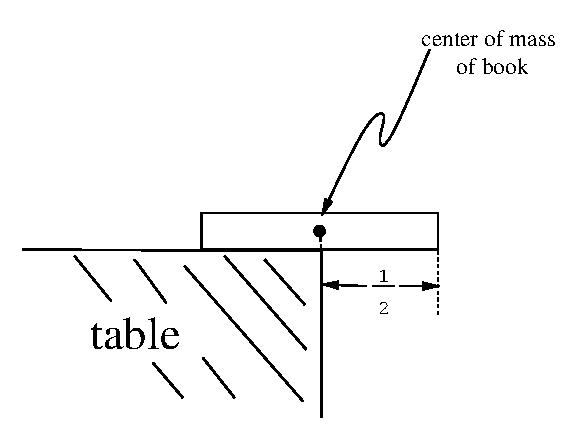
\includegraphics[width=.40\textwidth]{figures/bookstack-3}}
\caption{One book can overhang half a book length.}
\label{one-stable-book}
\end{figure}

Now suppose we have a stack of books that will stick out past the table
edge without tipping over---call that a \emph{stable} stack.  Let's define
the \term{overhang} of a stable stack to be the largest horizontal
distance from the center of mass of the stack to the furthest edge of a
book.  If we place the center of mass of the stable stack at the edge of
the table as in Figure~\ref{overhang}, that's how far we can get a book in
the stack to stick out past the edge.

\begin{figure}
\centerline{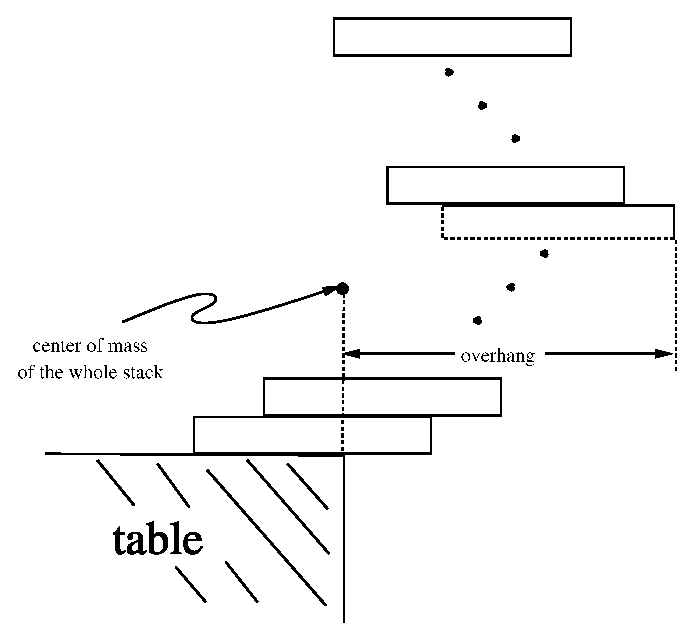
\includegraphics[width=.4\textwidth]{figures/bookstack-2}}
%\centerline{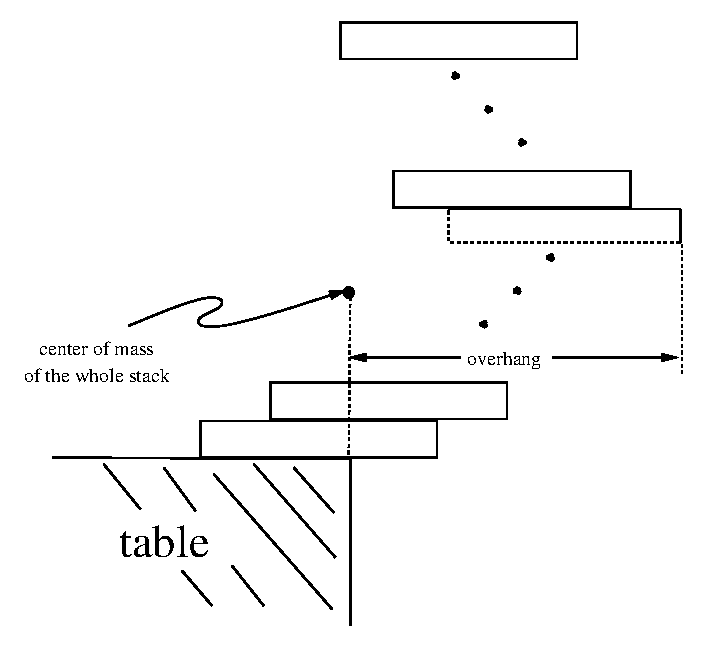
\psfig{file=figures/bookstack-2.ps,width=.4\textwidth}}
\caption{Overhanging the edge of the table.}
\label{overhang}
\end{figure}

So we want a formula for the maximum possible overhang, $B_n$, achievable
with a stack of $n$~books.

We've already observed that the overhang of one book is~1/2 a book
length.  That is,
\[
    B_1 = \frac{1}{2}.
\]

Now suppose we have a stable stack of $n+1$ books with maximum overhang.
If the overhang of the $n$ books on top of the bottom book was not
maximum, we could get a book to stick out further by replacing the top
stack with a stack of $n$ books with larger overhang.  So the maximum
overhang, $B_{n+1}$, of a stack of $n+1$ books is obtained by placing a
maximum overhang stable stack of $n$ books on top of the bottom book.  And
we get the biggest overhang for the stack of $n+1$ books by placing the
center of mass of the $n$ books right over the edge of the bottom book as
in Figure~\ref{Bn1}.

So we know where to place the $n+1$st book to get maximum overhang, and
all we have to do is calculate what it is.  The simplest way to do that is
to let the center of mass of the top $n$ books be the origin.  That way
the horizontal coordinate of the center of mass of the whole stack of
$n+1$ books will equal the increase in the overhang.  But now the
center of mass of the bottom book has horizontal coordinate $1/2$, so the
horizontal coordinate of center of mass of the whole stack of $n+1$ books is
\[
\frac{0 \cdot n + (1/2) \cdot 1}{n+1} = \frac{1}{2(n +1)}.
\]

In other words, 
\begin{equation}\label{eqBn}
    B_{n+1} = B_n + \frac{1}{2(n+1)},
\end{equation}
as shown in Figure~\ref{Bn1}.

\begin{figure}
\centerline{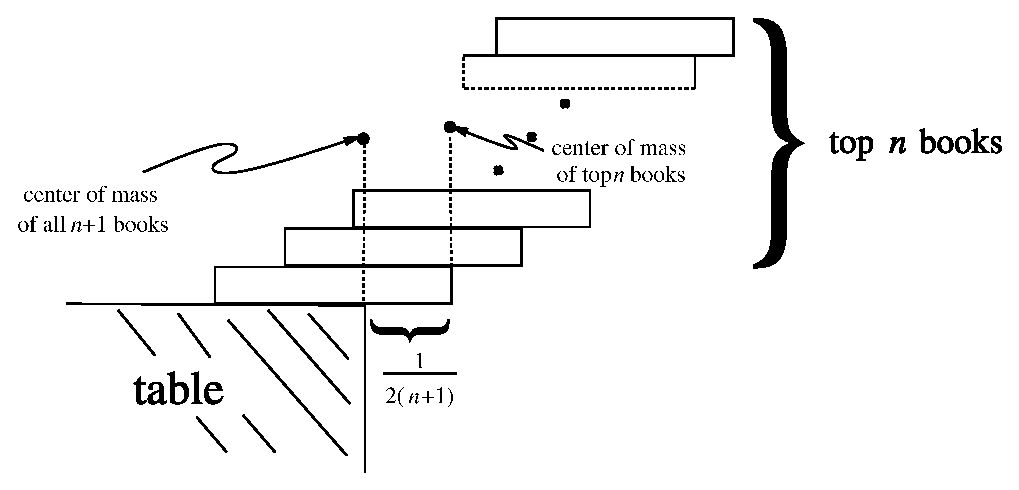
\includegraphics[width=.80\textwidth]{figures/bookstack-5}}
%\centerline{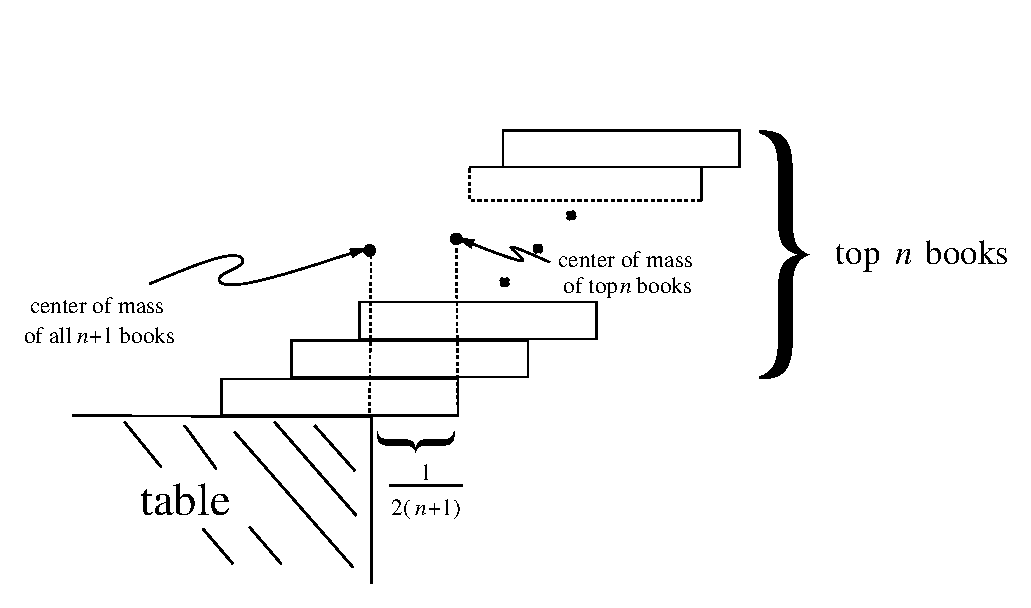
\psfig{file=figures/bookstack-5.ps,width=.80\textwidth}}
\caption{Additional overhang with $n+1$ books.}
\label{Bn1}
\end{figure}

Expanding equation~(\ref{eqBn}), we have
\begin{align}
B_{n+1} & = B_{n-1} + \frac{1}{2n} + \frac{1}{2(n+1)}\notag\\
        & = B_1 + \frac{1}{2 \cdot 2} + \cdots + \frac{1}{2n} +
            \frac{1}{2(n+1)}\notag\\
        & = \frac{1}{2}\sum_{i=1}^{n+1} \frac{1}{i}.\label{Bn+1sum}
\end{align}
The $n$th \term{Harmonic number}, $H_n$, is defined to be
\begin{definition}
\[
H_n \eqdef \sum_{i=1}^n \frac{1}{i}.
\]
\end{definition}
So~\eqref{Bn+1sum} means that
\[
B_n = \frac{H_n}{2}.
\]

The first few Harmonic numbers are easy to compute.  For example, $H_4 = 1
+ \frac{1}{2} + \frac{1}{3} + \frac{1}{4} = \frac{25}{12}$.  The fact that
$H_4$ is greater than 2 has special significance; it implies that the
total extension of a 4-book stack is greater than one full book!  This is
the situation shown in Figure~\ref{fig:optstack}.

\begin{figure}[htbp]
\centerline{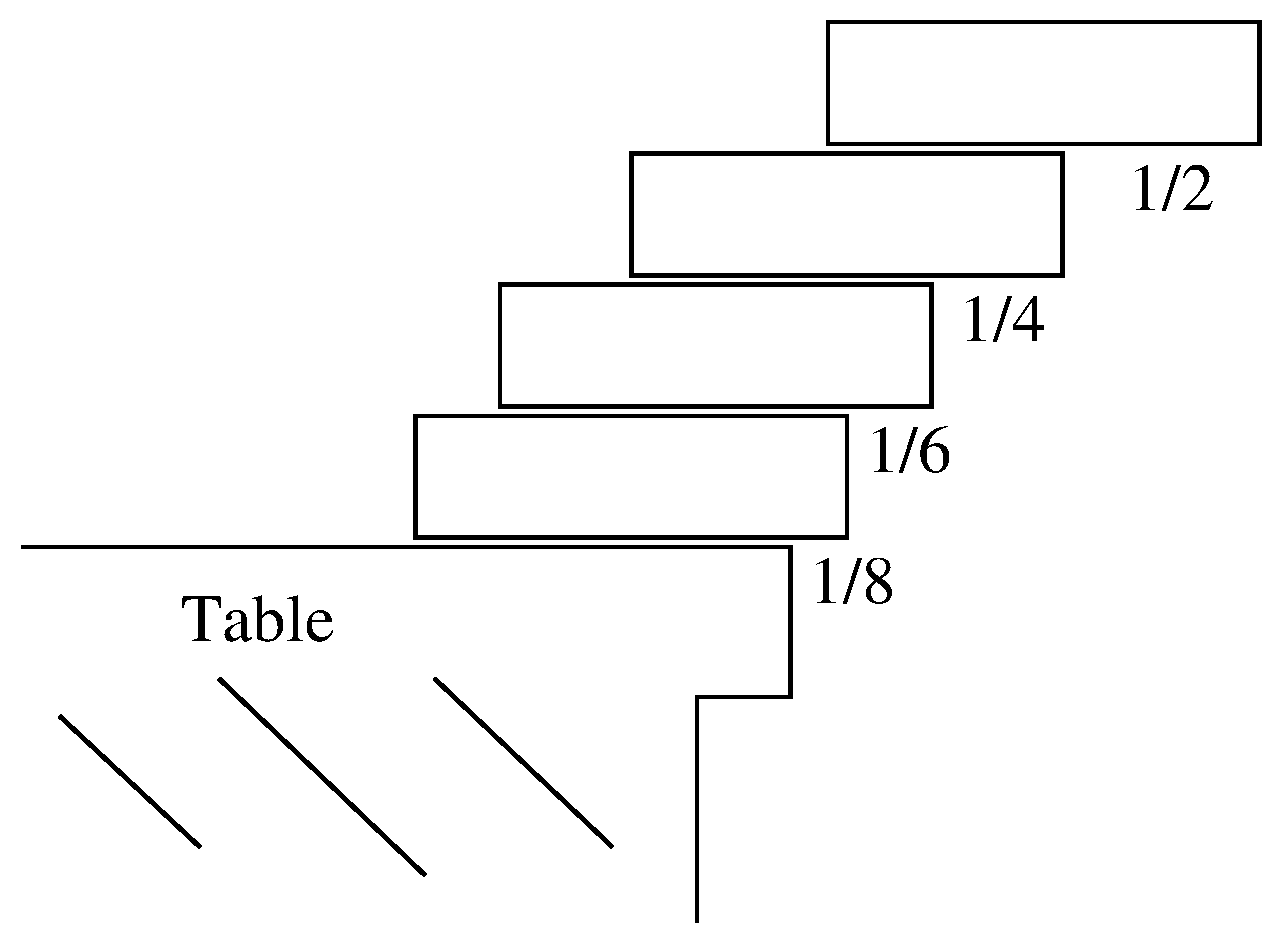
\includegraphics[height=1.5in]{figures/optstack}}
\caption{Stack of four books with maximum overhang.}
\label{fig:optstack}
\end{figure}

\hyperdef{integral}{method}{\subsection{Evaluating the Sum---The
    \idx{Integral Method}}}

It would be nice to answer questions like, ``How many books are needed
to build a stack extending 100 book lengths beyond the table?''  One
approach to this question would be to keep computing Harmonic numbers
until we found one exceeding 200.  However, as we will see, this is
not such a keen idea.

Such questions would be settled if we could express $H_n$ in a \idx{closed
  form}.  Unfortunately, no closed form is known, and probably none
exists.  As a second best, however, we can find closed forms for very good
\idx{approximations} to $H_n$ using the Integral Method.  The idea of the
Integral Method is to bound terms of the sum above and below by simple
functions as suggested in Figure~\ref{fig:integral}.  The integrals of
these functions then bound the value of the sum above and below.

\begin{figure}[htbp]
\centerline{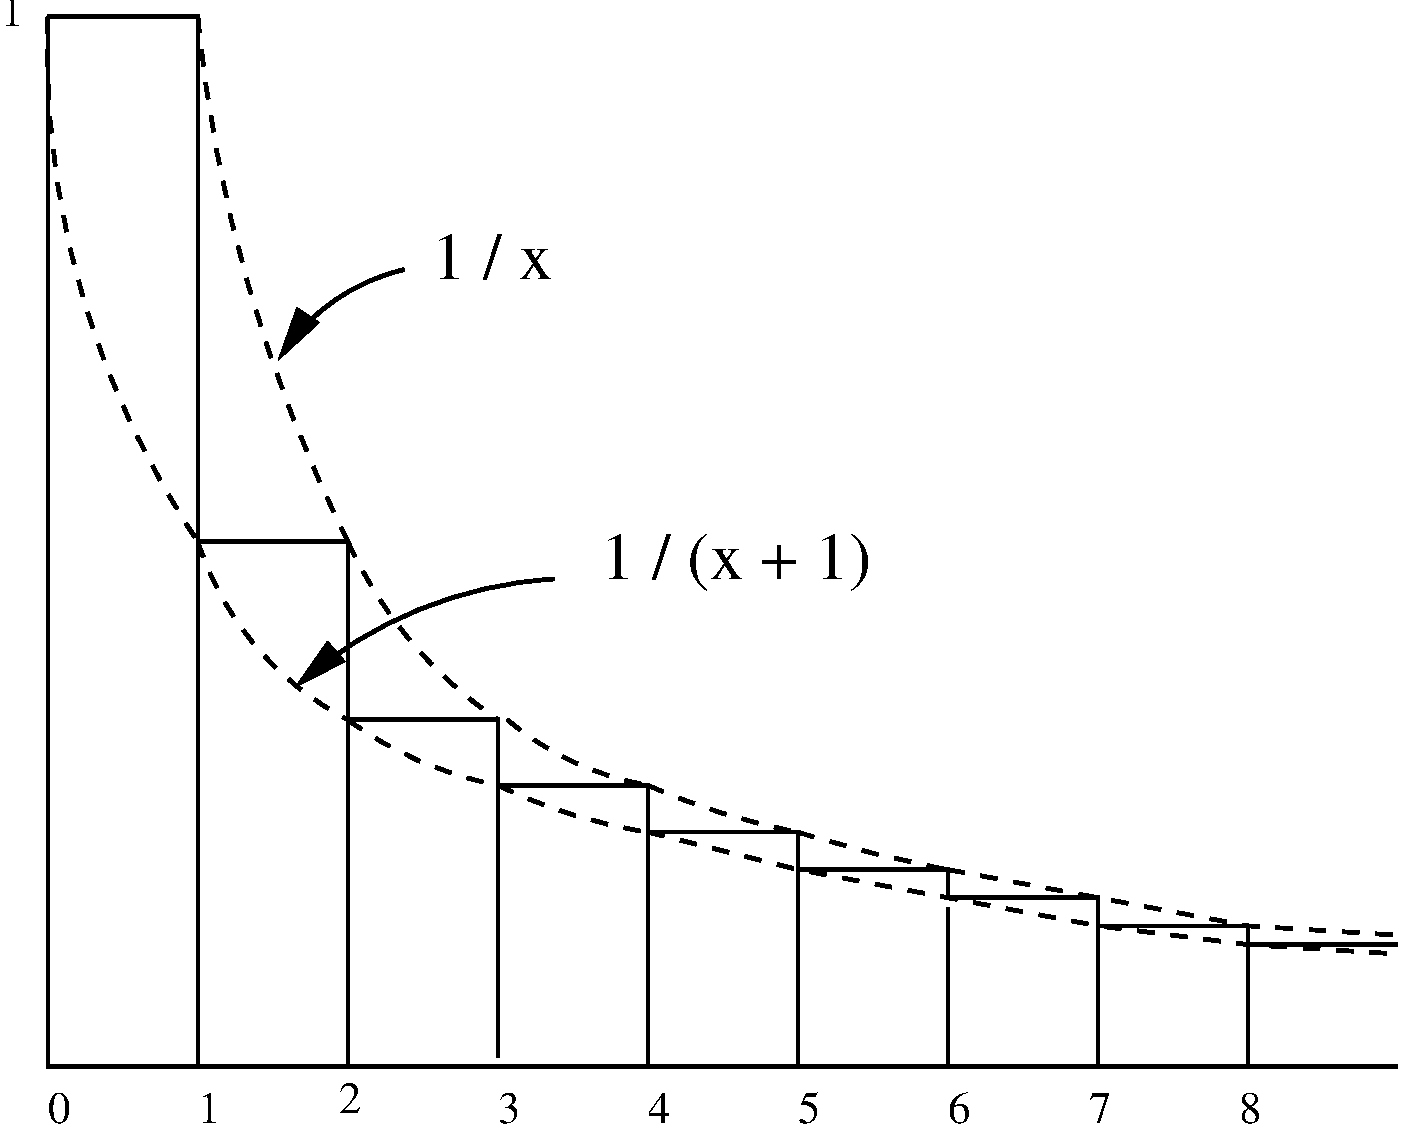
\includegraphics[height=2.0in]{figures/integral}}
\caption{\em This figure illustrates the Integral Method for bounding
a sum.  The area under the ``stairstep'' curve over the interval $[0,
n]$ is equal to $H_n = \sum_{i=1}^n 1/i$.  The function $1/x$ is
everywhere greater than or equal to the stairstep and so the integral
of $1/x$ over this interval is an upper bound on the sum.  Similarly,
$1/(x+1)$ is everywhere less than or equal to the stairstep and so the
integral of $1/(x+1)$ is a lower bound on the sum.}
\label{fig:integral}
\end{figure}

The Integral Method gives the following upper and lower bounds on the
harmonic number $H_n$:
\begin{eqnarray}
H_n & \leq & 1 + \int_1^n \frac{1}{x} \ dx = 1 + \ln n \label{Hnl}\\
H_n & \geq & \int_0^n \frac{1}{x+1} \ dx = \int_1^{n+1} \frac{1}{x} \ dx = \ln(n+1).\label{Hng}
\end{eqnarray}
These bounds imply that the harmonic number $H_n$ is around $\ln n$.

But $\ln n$ grows ---slowly ---but without bound.  That means we can get
books to overhang \emph{any distance} past the edge of the table by piling
them high enough!  For example, to build a stack extending three book
lengths beyond the table, we need a number of books $n$ so that $H_n \ge
6$.  By inequality~\eqref{Hng}, this means we want
\[
H_n \geq \ln(n+1) \geq 6,
\]
so $n \geq e^6-1$ books will work, that is, 403 books will be enough to
get a three book overhang.  Actual calculation of $H_6$ shows that 227
books is the smallest number that will work.

\subsection{More about Harmonic Numbers}

In the preceding section, we showed that $H_n$ is about $\ln n$.  An
even better approximation is known:
\[
H_n = \ln n + \gamma + \frac{1}{2n} + \frac{1}{12n^2} +
        \frac{\epsilon(n)}{120n^4}
\]
Here $\gamma$ is a value $0.577215664\dots$ called \term{Euler's
  constant}, and $\epsilon(n)$ is between 0 and 1 for all $n$.  We will
not prove this formula.

\subsubsection{Asymptotic Equality}
The shorthand $H_n \sim \ln n$ is used to indicate that the leading
term of $H_n$ is $\ln n$.  More precisely:
\begin{definition}\label{def:sim}
  For functions $f,g: \reals \to \reals$, we say $f$ is \index{$\sim$
    (asymptotic equality)}\term{asymptotically equal} to $g$, in symbols,
\[
f(x) \sim g(x)
\]
iff
\[
\lim_{x \rightarrow \infty} f(x)/g(x) = 1.
\]
\end{definition}

It's tempting to might write $H_n \sim \ln n + \gamma$ to indicate the two
leading terms, but it is not really right.  According to
Definition~\ref{def:sim}, $H_n \sim \ln n + c$ where $c$ is \emph{any
  constant}.  The correct way to indicate that $\gamma$ is the
second-largest term is $H_n - \ln n \sim \gamma$.

The reason that the $\sim$ notation is useful is that often we do not care
about lower order terms.  For example, if $n = 100$, then we can compute
$H(n)$ to great precision using only the two leading terms:
\[
\abs{H_n - \ln n - \gamma} \leq \abs{\frac{1}{200} - \frac{1}{120000} +
\frac{1}{120 \cdot 100^4}} < \frac{1}{200}.
\]
\begin{problems}
\classproblems
\pinput{CP_holy_grail}
\pinput{CP_harmonic_number_divergence}

\homeworkproblems
\pinput{PS_bug_on_rug_harmonic_number}

\end{problems}
\section{Finding Summation Formulas}\label{findsum_sec}

The Integral Method offers a way to derive formulas like those
for the sum of consecutive integers,
\[
\sum_{i=1}^n i = n(n+1)/2,
\]
or for the sum of squares,
\begin{align}
\sum_{i=1}^n i^2 & =  \frac{(2n+1)(n+1)n}{6}\notag \\
                & =  \frac{n^3}{3} + \frac{n^2}{2} + \frac{n}{6}.\label{sumsqcubic}
%                 & \sim & \frac{n^3}{3}.
\end{align}

These equations appeared in Chapter~\ref{well_ordering_chap} as
equations~\eqref{sum1n} and~\eqref{sum-of-sq} where they were proved using
the Well-ordering Principle.  But those proofs did not explain how someone
figured out in the first place that these were the formulas to prove.

Here's how the Integral Method leads to the sum-of-squares formula, for
example.  First, get a quick estimate of the sum:
\[
\int_0^n x^2 \ dx \leq \sum_{i=1}^n i^2 \leq \int_0^n (x+1)^2 \ dx,
\]
so
\begin{equation}\label{n33leq}
n^3/3     \leq \sum_{i=1}^n i^2 \leq (n+1)^3/3 - 1/3.
\end{equation}
and the upper and lower bounds~\eqref{n33leq} imply that
\[
\sum_{i=1}^n i^2 \sim n^3/3.
\]
To get an exact formula, we then guess the general form of the solution.
Where we are uncertain, we can add parameters $a, b, c, \dots$.  For
example, we might make the guess:
\[
\sum_{i=1}^n i^2 = an^3 + bn^2 + cn + d.
\]
If the guess is correct, then we can determine the parameters $a$,
$b$, $c$, and $d$ by plugging in a few values for $n$.  Each such
value gives a linear equation in $a$, $b$, $c$, and $d$.  If we plug
in enough values, we may get a linear system with a unique solution.
Applying this method to our example gives:
\begin{align*}
n = 0 & \qimplies  0 = d \\
n = 1 & \qimplies  1 = a + b + c + d \\
n = 2 & \qimplies  5 = 8a + 4b + 2c + d \\
n = 3 & \qimplies  14 = 27a + 9b + 3c + d.
\end{align*}
Solving this system gives the solution $a = 1/3$, $b = 1/2$, $c = 1/6$, $d
= 0$.  Therefore, \emph{if} our initial guess at the form of the solution
was correct, then the summation is equal to $n^3/3 + n^2/2 + n/6$, which
matches equation~\eqref{sumsqcubic}.

The point is that if the desired formula turns out to be a polynomial,
then once you get an estimate of the \emph{degree} of the polynomial ---by
the Integral Method or any other way ---all the coefficients of the
polynomial can be found automatically.

\textbf{Be careful!}  This method let's you discover formulas, but it
doesn't guarantee they are right!  After obtaining a formula by this
method, it's important to go back and \emph{prove} it using induction or
some other method, because if the initial guess at the solution was not of
the right form, then the resulting formula will be completely wrong!

\subsection{Double Sums}

Sometimes we have to evaluate sums of sums, otherwise known as
\term{double summations}.  This can be easy: evaluate the inner
sum, replace it with a closed form, and then evaluate the outer sum which
no longer has a summation inside it.  For example,
\begin{align*}
\lefteqn{\sum_{n=0}^{\infty} \paren{y^n \sum_{i=0}^n x^i}}\\
 & = \sum_{n=0}^{\infty} \paren{y^n \frac{1-x^{n+1}}{1-x}}
     & \text{(geometric sum formula~\eqref{geometric-sum-n-1})}\\
 & = \frac{\sum_{n=0}^{\infty} y^n}{1-x} - \frac{\sum_{n=0}^{\infty} y^nx^{n+1}}{1-x}\\
 & = \frac{1}{(1-y)(1-x)} - \frac{x\sum_{n=0}^{\infty} \paren{xy}^n}{1-x}
      & \text{(infinite geometric sum, Theorem~\ref{th:series})}\\
 & = \frac{1}{(1-y)(1-x)} - \frac{x}{(1-xy)(1-x)}
      & \text{(infinite geometric sum, Theorem~\ref{th:series})}\\
  & = \frac{\paren{1-xy} - x(1-y)}{(1-xy)(1-y)(1-x)}\\
  & = \frac{1-x}{(1-xy)(1-y)(1-x)}\\
  & = \frac{1}{(1-xy)(1-y)}.
\end{align*}

When there's no obvious closed form for the inner sum, a special trick
that is often useful is to try \emph{exchanging the order of summation.}
For example, suppose we want to compute the sum of the harmonic numbers
\[
\sum_{k=1}^n H_k = \sum_{k=1}^n \sum_{j=1}^k 1/j
\]
For intuition about this sum, we can try the integral method:
\[
\sum_{k=1}^n H_k \approx \int_{1}^n \ln x \ dx \approx n\ln n-n.
\]

Now let's look for an exact answer.  If we think about the pairs
$(k,j)$ over which we are summing, they form a triangle:
\[
\begin{array}{cc|ccccccc}
 &  & j &   &   &   &   &       &   \\
 &  & 1 & 2 & 3 & 4 & 5 & \dots & n \\
\hline
k & 1 & 1\\
  & 2 &1&1/2\\
  & 3 &1&1/2&1/3\\
  & 4 &1&1/2&1/3&1/4\\
  &   &\dots\\
  & n &1&1/2&&\dots&&&1/n
\end{array}
\]
The summation above is summing each row and then adding the row sums.
Instead, we can sum the columns and then add the column sums.
Inspecting the table we see that this double sum can be written as
\begin{align}
\sum_{k=1}^n H_k &= \sum_{k=1}^n \sum_{j=1}^k 1/j\notag\\
&= \sum_{j=1}^n \sum_{k=j}^n 1/j\notag\\
&= \sum_{j=1}^n 1/j \sum_{k=j}^n 1\notag\\
&= \sum_{j=1}^n \frac1j (n-j+1)\notag\\
&= \sum_{j=1}^n \frac{n-j+1}j \notag\\
&= \sum_{j=1}^n \frac{n+1}j - \sum_{j=1}^n \frac{j}{j}\notag\\
&= (n+1)\sum_{j=1}^n \frac1j - \sum_{j=1}^n 1\notag\\
&= (n+1)H_n-n.\label{sHk}
\end{align}

\section{Stirling's Approximation}\label{Stirling_sec}

The familiar \idx{factorial} notation, $n!$, is an abbreviation for the
product
\[
\prod_{i=1}^n i.
\]
This is by far the most common product in discrete mathematics.  In this
section we describe a good closed-form estimate of $n!$ called
\term{Stirling's Approximation}.  Unfortunately, all we can do is
estimate: there is no closed form for $n!$ ---though proving so would take
us beyond the scope of 6.042.

\subsection{Products to Sums}

A good way to handle a product is often to convert it into a sum by taking
the logarithm.  In the case of factorial, this gives
\begin{align*}
\ln (n!) 
       & =  \ln(1 \cdot 2 \cdot 3 \cdots (n-1) \cdot n) \\
       & =  \ln 1 + \ln 2 + \ln 3 + \cdots + \ln(n-1) + \ln n \\
       & =  \sum_{i=1}^n \ln i.
\end{align*}
We've not seen a summation containing a \idx{logarithm} before!
Fortunately, one tool that we used in evaluating sums is still applicable:
the \idx{Integral Method}.  We can bound the terms of this sum with $\ln
x$ and $\ln(x+1)$ as shown in Figure~\ref{fig:integral2}.  This gives
bounds on $\ln(n!)$ as follows:
\begin{eqnarray*}
\int_1^n \ln x \ dx \leq & \sum_{i=1}^n \ln i & \leq \int_0^n \ln(x+1) \ dx \\
n \ln(\frac{n}{e}) + 1 \leq & \sum_{i=1}^n \ln i & \leq (n+1) \ln\paren{\frac{n+1}{e}} + 1 \\
\paren{\frac{n}{e}}^n e \leq & n! & \leq  \paren{\frac{n+1}{e}}^{n+1} e.
\end{eqnarray*}
The second line follows from the first by completing the integrations.
The third line is obtained by exponentiating.

\begin{figure}[htbp]
\centerline{%
%\psfig{figure=figures/integral2.eps,height=2in}
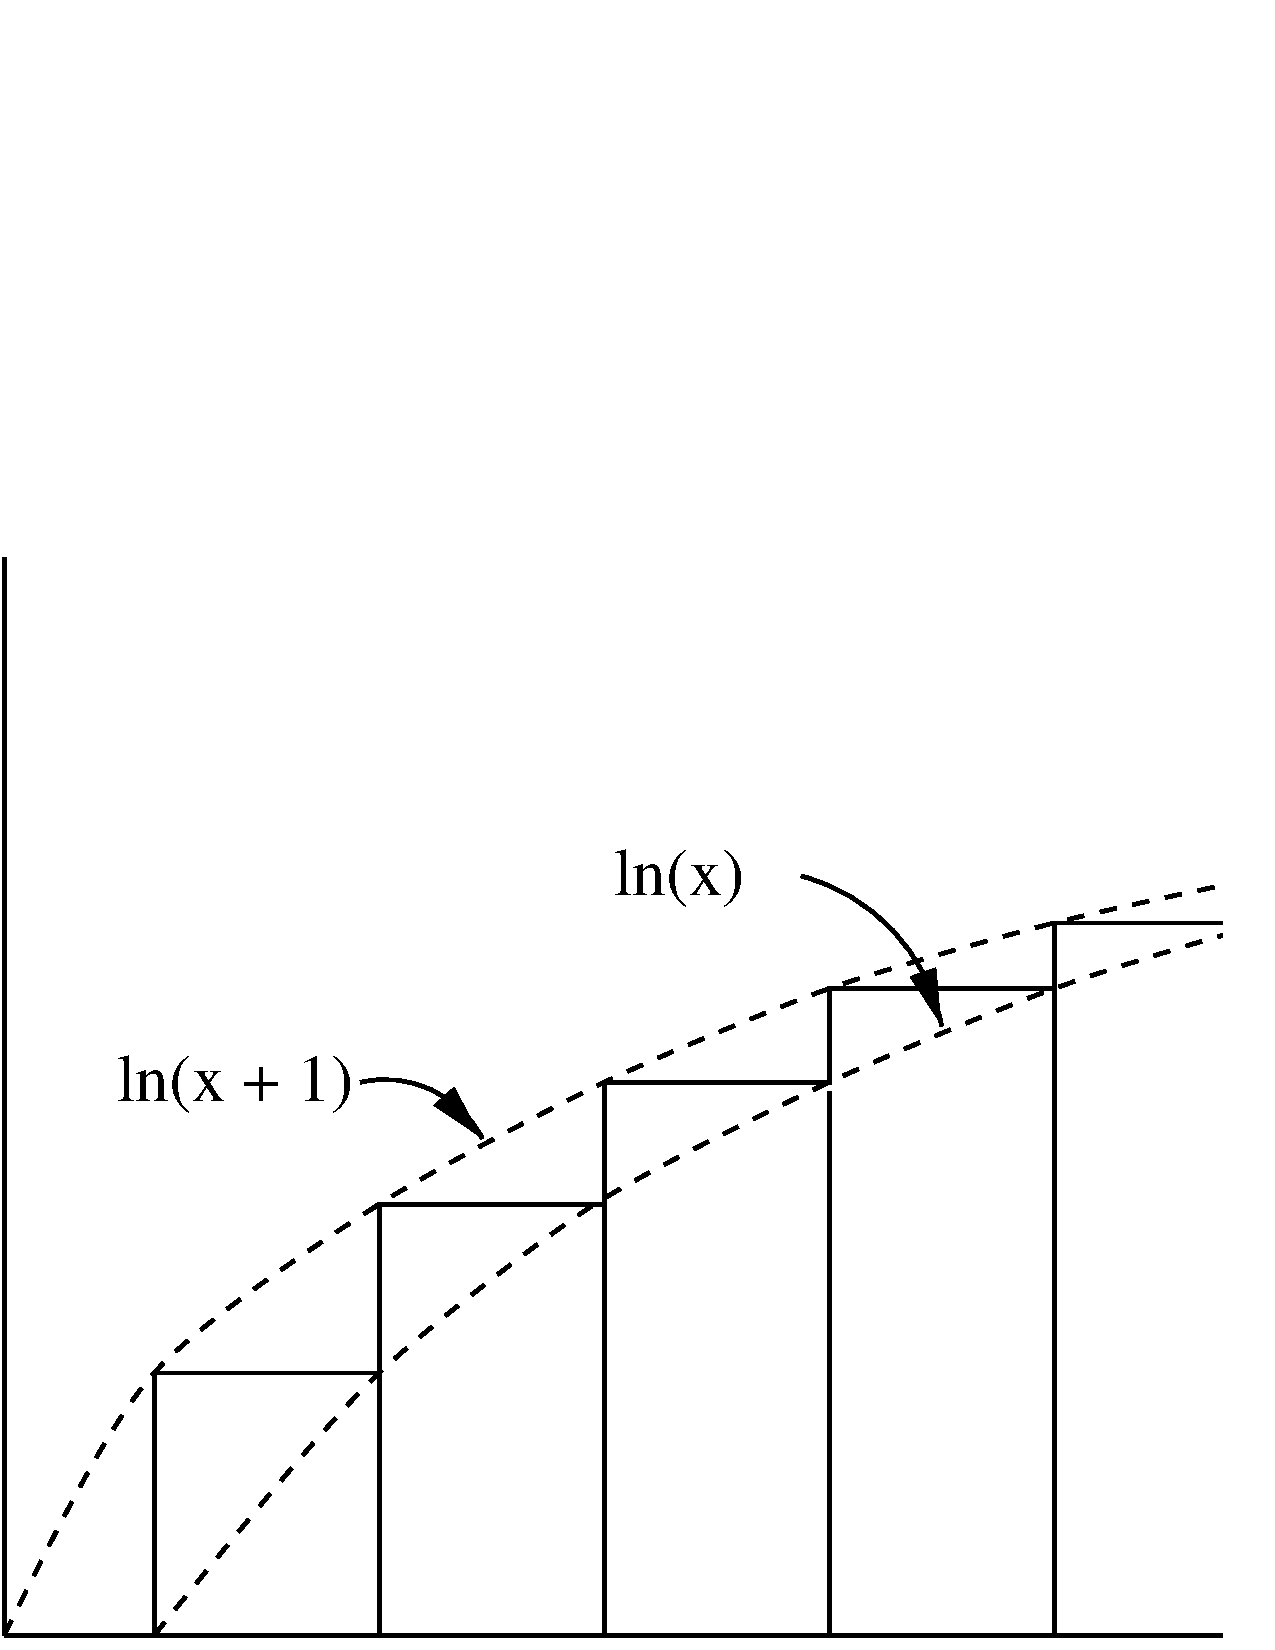
\includegraphics[height=2in]{figures/integral2}
}
\caption{\em This figure illustrates the Integral Method for bounding
the sum $\sum_{i=1}^n ln \ i$.}
\label{fig:integral2}
\end{figure}

So $n!$ behaves something like the closed form formula $(n/e)^n$.
A more careful analysis yields an unexpected closed form formula that is
asymptotically exact:
\begin{lemma*}[Stirling's Formula]
\begin{equation}\label{nfacsim}
n! \sim \left(\frac{n}{e}\right)^n \sqrt{2 \pi n},
\end{equation}
\end{lemma*}

\idx{Stirling's Formula} describes how $n!$ behaves in the limit, but to
use it effectively, we need to know how close it is to the limit for
different values of $n$.  That information is given by the bounding
formulas:
\begin{fact*}[Stirling's Approximation]
\[
\sqrt{2 \pi n} \left(\frac{n}{e}\right)^n e^{1/(12n+1)} \leq n! \leq
\sqrt{2 \pi n} \left(\frac{n}{e}\right)^n e^{1/12n}.
\]
\end{fact*}
\idx{Stirling's Approximation} implies the asymptotic
formula~\eqref{nfacsim}, since $e^{1/(12n+1)}$ and $e^{1/12n}$ both
approach 1 as $n$ grows large.  These inequalities can be verified by
induction, but the details are nasty.

The bounds in Stirling's formula are very tight.  For example, if $n =
100$, then Stirling's bounds are:
\begin{align*}
100! & \geq  \sqrt{200 \pi} \left(\frac{100}{e}\right)^{100} e^{1/1201} \\
100! & \leq  \sqrt{200 \pi} \left(\frac{100}{e}\right)^{100} e^{1/1200}
\end{align*}

The only difference between the upper bound and the lower bound is in
the final term.  In particular $e^{1/1201} \approx 1.00083299$ and
$e^{1/1200} \approx 1.00083368$.  As a result, the upper bound is no
more than $1 + 10^{-6}$ times the lower bound.  This is amazingly
tight!  Remember Stirling's formula; we will use it often.

\begin{staffnotes}

\subsection*{Bounds by Double Summing}

Another way to derive Stirling's approximation is to remember that
$\ln n$ is roughly the same as $H_{n}$.  This lets us use the result
we derived before for $\sum H_k$ via double summation.  Our
approximation for $H_k$ told us that $\ln(k+1)\le H_k \le 1+\ln k$.
Rewriting, we find that $H_{k}-1 \le \ln k \le H_{k - 1}$.  It follows
that (leaving out the $i=1$ term in the sum, which contributes 0),
\begin{align*}
\sum_{i=2}^n \ln i &\le  \sum_{i=2}^n H_{i-1}\\
&= \sum_{i=1}^{n-1} H_i\\
&= nH_{n-1}-(n-1) & \text{by~(\ref{sHk})}\\
&\le n(1+\ln(n-1))-(n-1) & \text{by~(\ref{Hnl})}\\\\
&=n\ln(n-1)+1,
\end{align*}
roughly the same bound as we proved before via the integral method.
We can derive a similar lower bound.

\end{staffnotes}

\hyperdef{asymptotic}{notation}{\section{Asymptotic
    Notation}}\label{asymptotic_sec}

Asymptotic notation is a shorthand used to give a quick measure of the
behavior of a function $f(n)$ as $n$ grows large.

\subsection{\index{o(), little oh}Little Oh}

The asymptotic notation, \idx{$\sim$}, of Definition~\ref{def:sim} is a
binary relation indicating that two functions grow at the \emph{same}
rate.  There is also a binary relation indicating that one function grows
at a significantly \emph{slower} rate than another.  Namely,
\begin{definition}
  For functions $f,g: \reals \to \reals$, with $g$ nonnegative, we say $f$
  is \index{o(), asymptotically smaller}\term{asymptotically smaller} than
  $g$, in symbols,
\[
f(x) = o(g(x)),
\]
iff
\[
\lim_{x \rightarrow \infty} f(x)/g(x) = 0.
\]
\end{definition}

For example, $1000x^{1.9} = o(x^2)$, because $1000x^{1.9}/x^2 =
1000/x^{0.1}$ and since $x^{0.1}$ goes to infinity with $x$ and 1000 is
constant, we have $\lim_{x \rightarrow \infty} 1000x^{1.9}/x^2 = 0$.
This argument generalizes directly to yield
\begin{lemma}\label{xaoxb}
$x^a = o(x^b)$ for all nonnegative constants $a<b$.
\end{lemma}

Using the familiar fact that  $\log x < x$ for all $x >1$, we can prove
\begin{lemma}\label{logxxe}
$\log x = o(x^{\epsilon})$ for all $\epsilon >0$ and $x > 1$.
\end{lemma}

\begin{proof}
Choose $\epsilon > \delta > 0$ and let $x = z^\delta$ in the inequality
$\log x < x$.  This implies
\begin{equation}\label{zdd}
\log z  <  z^{\delta}/\delta
 =  o(z^{\epsilon})\qquad \text{by Lemma~\ref{xaoxb}}.
\end{equation}
\end{proof}

\begin{corollary}\label{xbax}
$x^b = o(a^x)$ for any $a,b \in \reals$ with $a>1$.
\end{corollary}

\begin{proof}
From~(\ref{zdd}),
\[   %\begin{equation}\label{dd}
\log z  <  z^{\delta}/\delta
\]   %\end{equation}
for all $z>1$, $\delta >0$.  
Hence
\begin{align*}
(e^b)^{\log z} & <  (e^b)^{z^{\delta}/\delta}\\ %\notag\\
z^b & < \paren{e^{\log a (b/\log a)}}^{z^{\delta}/\delta}\\ %\notag\\
    & =  a^{(b/\delta\log a) z^{\delta}}\\ %\notag\\
    & <  a^z  %\label{az}
\end{align*}
for all $z$ such that
\[
(b/\delta\log a) z^{\delta} <z.
\]
But choosing $\delta < 1$, we know $z^{\delta} = o(z)$, so this last
inequality holds for all large enough $z$.
\end{proof}

Lemma~\ref{logxxe} and Corollary~\ref{xbax} can also be proved easily in
several other ways, for example, using L'Hopital's Rule or the McLaurin
Series for $\log x$ and $e^x$.  Proofs can be found in most calculus
texts.

\subsection{\index{O(), big oh}Big Oh}

Big Oh is the most frequently used asymptotic notation.  It is used to
give an upper bound on the growth of a function, such as the running
time of an algorithm.
\begin{definition}
Given nonnegative functions $f, g : \reals \to \reals$, we
say that
\[
f = O(g)
\]
iff
\[
\limsup_{x \rightarrow \infty} f(x)/g(x) < \infty.
\]
\end{definition}
This definition\footnote{We can't simply use the limit as
$x \rightarrow \infty$ in the definition of $O()$, because if
$f(x)/g(x)$ oscillates between, say, 3 and 5 as $x$ grows, then $f =
O(g)$ because $f
\leq 5g$, but $\lim_{x \rightarrow \infty} f(x)/g(x)$ does not exist.
So instead of limit, we use the technical notion of $\limsup$.  In
this oscillating case, $\limsup_{x \rightarrow \infty} f(x)/g(x) = 5$.

The precise definition of $\limsup$ is
\[
\limsup_{x \rightarrow \infty} h(x) \eqdef \lim_{x \rightarrow \infty}
\text{lub}_{y \geq x} h(y),
\]
where ``lub'' abbreviates ``least upper bound.''} makes it clear that
\begin{lemma}\label{osimO}
If $f = o(g)$ or $f \sim g$, then $f = O(g)$.
\end{lemma}
\begin{proof}
$\lim f/g=0$ or $\lim f/g=1$ implies $\lim f/g<\infty$.
\end{proof}

It is easy to see that the converse of Lemma~\ref{osimO} is not true.  For
example, $2x = O(x)$, but $2x \not\sim x$ and $2x \neq o(x)$.

The usual formulation of Big Oh spells out the definition of $\limsup$
without mentioning it.  Namely, here is an equivalent definition:
\begin{definition}
Given functions $f, g : \reals \to \reals$, we say that
\[
f = O(g)
\]
iff there exists a constant $c \geq 0$ and an $x_0$ such that for all $x \geq
x_0$, $\abs{f(x)} \leq c g(x)$.
\end{definition}

This definition is rather complicated, but the idea is simple: $f(x) =
O(g(x))$ means $f(x)$ is less than or equal to $g(x)$, except that we're
willing to ignore a constant factor, namely, $c$, and to allow exceptions for
small $x$, namely, $x < x_0$.

We observe,
\begin{lemma}
If $f = o(g)$, then it is \emph{not} true that $g = O(f)$.
\end{lemma}
\begin{proof}
\[
\lim_{x \rightarrow \infty} \frac{g(x)}{f(x)} =
 \frac{1}{\lim_{x \rightarrow \infty} f(x)/g(x)} =
 \frac{1}{0} = \infty,
\]
so $g \neq O(f)$.

\iffalse
We will prove the equivalent contrapositive, i.e., that
if $g=O(f)$ then it is not true that $f=o(g)$.  If
$g=O(f)$ then there 
exists a constant $c \geq 0$ and an $x_0$ such that for all $x \geq
x_0$, $\abs{g(x)} \leq c f(x)$.
Then for all $x \geq x_0$, we have that $f(x)/|g(x)| = f(x)/g(x) >c>0$
(the first equality uses the nonnegativity of $g$).
Thus $\lim_{x \rightarrow \infty} f(x)/g(x) >0$ and so it is not true that
$f=o(g)$.
\fi

\end{proof}

\begin{proposition}
$100x^2 = O(x^2)$.
\end{proposition}

\begin{proof}
Choose $c = 100$ and $x_0 = 1$.  Then the proposition holds, since for all
$x \geq 1$, $\abs{100x^2} \leq 100 x^2$.
\end{proof}

\begin{proposition}\label{x2O}
$x^2 + 100x + 10 = O(x^2)$.
\end{proposition}

\begin{proof}
$(x^2 + 100x + 10)/x^2 = 1 + 100/x + 10/x^2$ and so its limit as $x$
approaches infinity is $1 + 0 + 0 = 1$.  So in fact, $x^2 + 100x + 10 \sim
x^2$, and therefore $x^2 + 100x + 10 = O(x^2)$.  Indeed, it's conversely
true that $x^2= O(x^2 + 100x + 10)$.
\end{proof}

Proposition~\ref{x2O} generalizes to an arbitrary polynomial:
\begin{proposition}
For $a_k\neq 0$, $a_k x^k + a_{k-1} x^{k-1} + \cdots + a_1x + a_0 = O(x^k)$.
\end{proposition}
We'll omit the routine proof.

Big Oh notation is especially useful when describing the running time of
an algorithm.  For example, the usual algorithm for multiplying $n \times
n$ matrices requires proportional to $n^3$ operations in the worst case.
This fact can be expressed concisely by saying that the running time is
$O(n^3)$.  So this asymptotic notation allows the speed of the algorithm
to be discussed without reference to constant factors or lower-order terms
that might be machine specific.  In this case there is another, ingenious
\idx{matrix multiplication} procedure that requires $O(n^{2.55})$
operations.  This procedure will therefore be much more efficient on large
enough matrices.  Unfortunately, the $O(n^{2.55})$-operation
multiplication procedure is almost never used because it happens to be
less efficient than the usual $O(n^3)$ procedure on matrices of practical
size. 
\begin{staffnotes}
It is even conceivable that there is an $O(n^2)$ matrix
multiplication procedure, but none is known.
\end{staffnotes}

\subsection{\index{$\Theta()$}Theta}

\begin{definition}
\[
f = \varTheta(g)
\qiff
f=O(g) \text{ and } g=O(f).
\]
\end{definition}

The statement $f = \varTheta(g)$ can be paraphrased intuitively as ``$f$
and $g$ are equal to within a constant factor.''

The value of these notations is that they highlight growth rates and allow
suppression of distracting factors and low-order terms.  For example, if
the running time of an algorithm is
\[
T(n) = 10n^3 - 20n^2 + 1,
\]
then
\[
T(n) = \varTheta(n^3).
\]
In this case, we would say that \emph{$T$ is of order $n^3$} or that
\emph{$T(n)$ grows cubically}.

Another such example is
\[
{{\pi^23^{x-7} + \frac{(2.7x^{113} + x^9- 86)^4}{\sqrt{x}} - 1.08^{3x}}} =
\varTheta(3^x).
\]

Just knowing that the running time of an algorithm is $\varTheta(n^3)$, for
example, is useful, because if $n$ doubles we can predict that the running
time will \emph{by and large}\footnote{Since $\varTheta(n^3)$ only implies
that the running time, $T(n)$, is between $cn^3$ and $dn^3$ for constants
$0<c<d$, the time $T(2n)$ could regularly exceed $T(n)$ by a factor as large
as $8d/c$.  The factor is sure to be close to 8 for all large $n$ only if
$T(n) \sim n^3$.} increase by a factor of at most $8$ for large $n$.  In
this way, Theta notation preserves information about the scalability of an
algorithm or system.  Scalability is, of course, a big issue in the design
of algorithms and systems.

\begin{staffnotes}

Figure~\ref{asymp} illustrates the relationships among the asymptotic
growth notations we have considered.

\begin{figure}[h]
\begin{center}
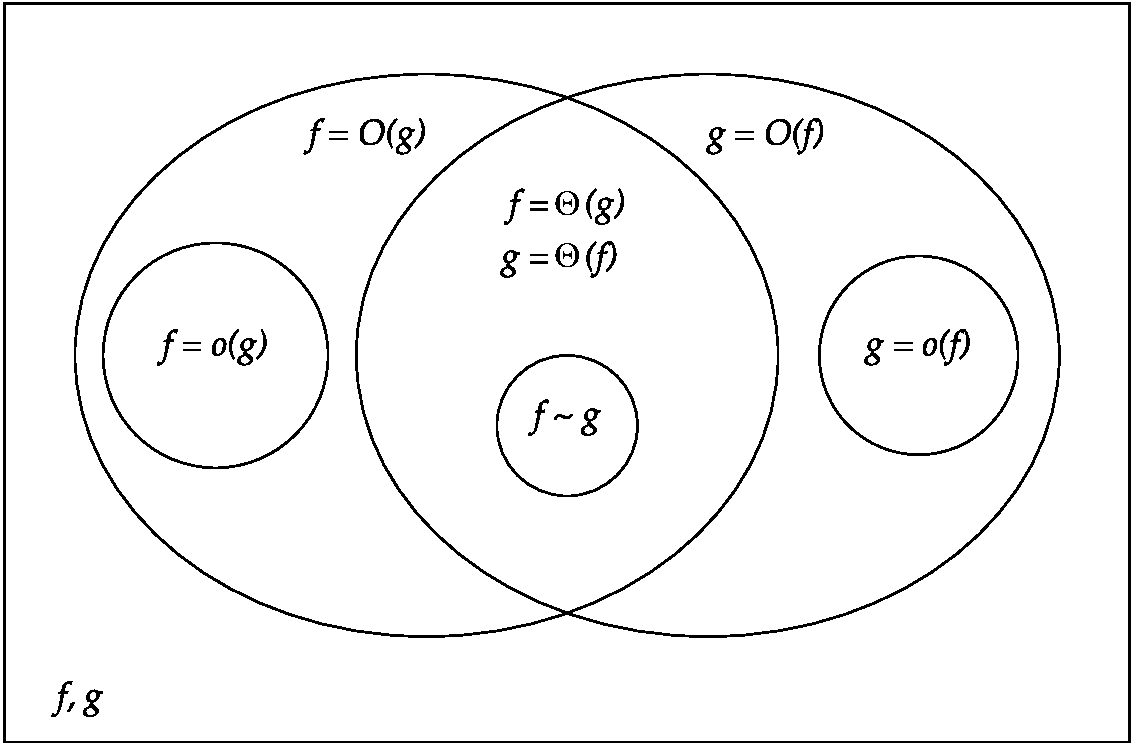
\includegraphics[width=6in]{figures/asymp}
\end{center}
\caption{Venn Diagram describing Asymptotic Relations}
\label{asymp}
\end{figure}

\end{staffnotes}


\subsection{Pitfalls with \idx{Big Oh}}

There is a long list of ways to make mistakes with Big Oh notation.
This section presents some of the ways that Big Oh notation can lead
to ruin and despair.

\subsubsection{The Exponential Fiasco}

Sometimes relationships involving Big Oh are not so obvious.  For
example, one might guess that $4^x = O(2^x)$ since 4 is only a
constant factor larger than 2.  This reasoning is incorrect,
however; actually $4^x$ grows much faster than $2^x$.

\begin{proposition}
$4^x \neq O(2^x)$
\end{proposition}

\begin{proof}
$2^x/4^x = 2^x/(2^x2^x) = 1/2^x$.  Hence, $\lim_{x \rightarrow \infty}
2^x/4^x = 0$, so in fact $2^x = o(4^x)$.  We observed earlier that this
implies that $4^x \neq O(2^x)$.
\end{proof}

\subsubsection{Constant Confusion}

Every constant is $O(1)$.  For example, $17 = O(1)$.  This is true because
if we let $f(x) = 17$ and $g(x) = 1$, then there exists a $c > 0$ and an
$x_0$ such that $\abs{f(x)} \leq c g(x)$.  In particular, we could choose
$c$ = 17 and $x_0 = 1$, since $\abs{17} \leq 17 \cdot 1$ for all $x \geq
1$.  We can construct a false theorem that exploits this fact.

\begin{falsethm}
\[
\sum_{i=1}^n i = O(n)
\]
\end{falsethm}

\begin{falseproof}
Define $f(n) = \sum_{i=1}^n i = 1 + 2 + 3 + \cdots + n$.  Since we
have shown that every constant $i$ is $O(1)$, $f(n) = O(1) + O(1) +
\cdots + O(1) = O(n)$.
\end{falseproof}

Of course in reality $\sum_{i=1}^n i = n(n+1)/2 \neq O(n)$.

The error stems from confusion over what is meant in the statement $i =
O(1)$.  For any \emph{constant} $i\in \naturals$ it is true that $i =
O(1)$.  More precisely, if $f$ is any constant function, then $f = O(1)$.
But in this False Theorem, $i$ is not constant but ranges over a set of
values 0,1,\dots,$n$ that depends on $n$.

And anyway, we should not be adding $O(1)$'s as though they were numbers.
We never even defined what $O(g)$ means by itself; it should only be used
in the context ``$f = O(g)$'' to describe a relation between functions $f$
and $g$.

\subsubsection{Lower Bound Blunder}

Sometimes people incorrectly use Big Oh in the context of a lower bound.
For example, they might say, ``The running time, $T(n)$, is at least
$O(n^2)$,'' when they probably mean something like ``$O(T(n)) = n^2$,'' or
more properly, ``$n^2 = O(T(n))$.''

\subsubsection{Equality Blunder}

The notation $f = O(g)$ is too firmly entrenched to avoid, but the use of
``='' is really regrettable.  For example, if $f = O(g)$, it seems quite
reasonable to write $O(g) = f$.  But doing so might tempt us to the
following blunder: because $2n = O(n)$, we can say $O(n) = 2n$.  But $n =
O(n)$, so we conclude that $n = O(n) = 2n$, and therefore $n = 2n$.  To
avoid such nonsense, we will never write ``$O(f) = g$.''

\begin{problems}
\practiceproblems
\pinput{MQ_asymptotics_table}

\homeworkproblems
\pinput{PS_little_oh_properties}
\pinput{PS_asymptotics_table}
\pinput{PS_Stirlings_and_log_n_factorial}

\classproblems
\pinput{CP_Theta_log_n_factorial}
%\pinput{CP_Stirlings_and_log_n_factorial}
\pinput{CP_big_oh_practice}
%\pinput{CP_asymptotic_equality_pitfall}
\pinput{CP_false_asymptotics_proof}
\pinput{FP_Oh_not_Theta}
\end{problems}

\endinput
